% !TEX root = ../main.tex

%----------------------------------------------------------------------------------------
% APPENDIX A
%----------------------------------------------------------------------------------------

\chapter{Appendix A - Survey questions} % Main appendix title

\label{ApendixA} % Change X to a consecutive letter; for referencing this appendix elsewhere, use \ref{AppendixX}

\subsection*{Introduction}

Welcome to the survey about software product documentation management.

With this anonymous survey, we aim to gather your view and needs regarding software documentation and knowledge structure for SCRUM teams.

This survey is part of a research project that is being conducted at ZHAW. With the results, I try to find solutions and an approach for solving issues within documentation structures and how to keep them up-to-date and available to the right stakeholders.

Thank you in advance for your participation in this survey.

Please do not hesitate to contact me if you have any questions or feedback.

Which existing techniques support SCRUM Team knowledge management

In the context of this research we discuss three different techniques to improve the collaboration and knowledge sharing in SCRUM teams:

- Role Based Information Highlighting in Documents
- Decision Logs Within a Mirrored Approach
- Infrastructure As Code (IaC)

An illustration is provided below:

\begin{figure}[h!]
\centering
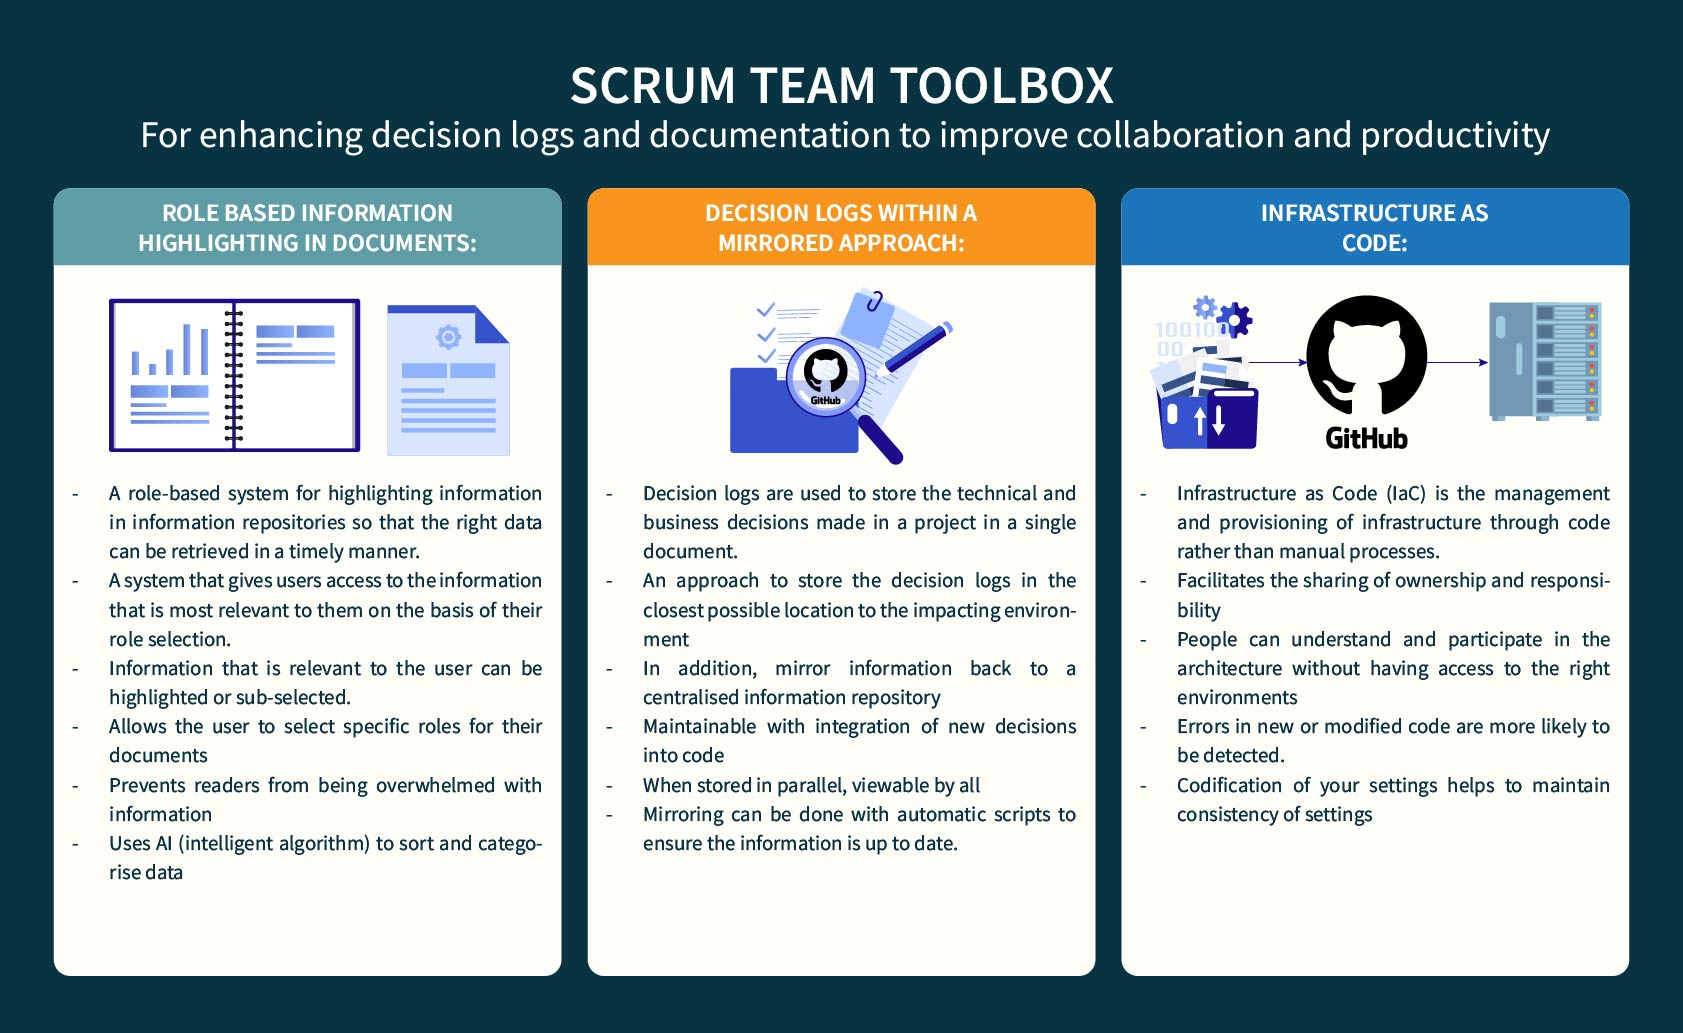
\includegraphics[width=\linewidth]{Images/toolbox.jpg}
\end{figure}

\newpage

\subsection*{Questions}
The following lists provide the questions for the survey. 


\subsubsection*{Demographics}

\textbf{Gender}
\begin{itemize}
    \item Male
    \item Female
    \item Other
\end{itemize}

\textbf{Your experience in the software engineering field?}
\begin{itemize}
    \item 0 Years
    \item 1 - 2 Years
    \item 3 - 5 Years
    \item 5 - 10 Years
    \item 10 + Years
\end{itemize}

\textbf{Your level of education or training in software engineering?}
\begin{itemize}
    \item No education / self-education or training
    \item Apprenticeship
    \item Higher Technical School (HF)
    \item Bachelor of Science or similar
    \item Master of Science or similar
    \item Doctor or similar
\end{itemize}

\textbf{Your role in a software development team that best suits you.}
\begin{itemize}
    \item Backend Engineer
    \item Frontend Engineer
    \item Full Stack Engineer
    \item Product Owner
    \item Business Analyst
    \item Quality Engineer
    \item UX Engineer
\end{itemize}

\textbf{Which software development paradigm is normally used in the projects you are involved with?}
\begin{itemize}
    \item Agile: Scrum, Kanban, XP, ...
    \item Traditional: Waterfall, Incremental Development, V-model, Spiral, ...
    \item Mixed
\end{itemize}

\subsubsection*{Role Based Information Highlighting in Documents}
A system should be developed that allows users to access only the information that is most relevant to their specific roles. This can be achieved by having users select the role that they perform on a daily basis. For example, a user who is a business analyst would select that as their role, whereas a user who is not would select a different role.

This system will ensure that team members do not become overwhelmed by unnecessary information. They will be able to focus on the information that pertains directly to their specific roles. This system should be maintained and ensured by an intelligent algorithm, or an AI model for short, which is configured for the right roles, and which is designed to highlight information that is based on the use of keywords in the text.

\textbf{Do you usually get overwhelmed by the amount of information when reading documentations?}
\begin{itemize}
    \item 1 (Not at all)
    \item \dots
    \item 10 (Very much)
\end{itemize}


\textbf{How satisfying would it be to have the information that is most important to you highlighted for you?}
\begin{itemize}
    \item 1 (Not at all)
    \item \dots
    \item 10 (Very much)
\end{itemize}

\textbf{How easy do you think it would be to use AI to automate the highlighting of information based on a viewer's role selection?}
\begin{itemize}
    \item 1 (Very easy)
    \item \dots
    \item 10 (Super hard)
\end{itemize}

\textbf{How much better do you think this approach of highlighting just the right information is than having separate pages for different roles?}
\begin{itemize}
    \item 1 (Not good at all!)
    \item \dots
    \item 10 (Very good idea!)
\end{itemize}

\textbf{In your personal experience, do you see people using more text or screenshots to document information?}
\begin{itemize}
    \item 1 (Only Screenshots)
    \item \dots
    \item 10 (Only Text)
\end{itemize}

\subsubsection*{Decision Logs Within a Mirrored Approach}
A system should be integrated that allows developers to utilize their decision logs in a logical manner. This would typically be at the closest possible distance to the affected source code, although in some cases, this may not be sufficient.
In addition, a way must be found to mirror this information into a single, centralised document that can be accessed by personnel from across the entire organisation or affected teams.

The new integration will ensure that the individuals responsible for integrating new decisions made by the teams are in proximity to the logs, enabling them to update them during the integration process.

On the other hand, it will reduce the time spent by developers on data mirroring to a centralized storage, which has frequently been identified as a challenge in maintaining document up-to-dateness.

\href{https://microsoft.github.io/code-with-engineering-playbook/design/design-reviews/decision-log/}{What are Decision Logs} 

\textbf{How important do you think it is to have a record of decisions and an up-to-date record of decisions?}
\begin{itemize}
    \item 1 (Not at all)
    \item \dots
    \item 10 (Super important)
\end{itemize}

\textbf{Did the decision logs you've seen so far contain the most up-to-date information, were they properly formatted and did they make sense?}
\begin{itemize}
    \item 1 (Not at all)
    \item \dots
    \item 10 (All of them)
\end{itemize}

\textbf{How do you think the decision logs would benefit from being part of the relevant code base, rather than a separate document, in terms of being up to date?}
\begin{itemize}
    \item 1 (Not at all)
    \item \dots
    \item 10 (Perfect Solution)
\end{itemize}

\textbf{How important do you think it is, if the decision logs are in the associated codebase, to still keep them in a document accessible to "non-developers"?}
\begin{itemize}
    \item 1 (Not important at all)
    \item \dots
    \item 10 (Very important)
\end{itemize}

\textbf{How easy do you think it would be to use tools to automate the mirroring of decisions into a separate document accessible to everyone?}
\begin{itemize}
    \item 1 (Very easy)
    \item \dots
    \item 10 (Super hard)
\end{itemize}

\subsubsection*{Infrastructure As Code (IaC)}

The objective of Infrastructure as Code is to facilitate consensus among the development team.

Tools such as Terraform are employed to this end. By automating the CI/CD process, the code that is incorporated into the 'main' branch of the project is subjected to rigorous examination during deployments and tests, which are all overseen by Infrastructure as Code.

Furthermore, the pods are recreated for E2E testing, thereby ensuring the availability of a realistic test environment that is closely aligned with the production environment.

\href{https://www.terraform.io/}{Terraform} 
\href{https://www.redhat.com/en/topics/automation/what-is-infrastructure-as-code-iac}{What is Infrastructure as Code (IaC)?} 


\textbf{In your current software project, how much do you know about how deployments and architectures work?}
\begin{itemize}
    \item 1 (No plan at all)
    \item \dots
    \item 10 (Deployed it myself)
\end{itemize}

\textbf{How familiar are you with the concept of Infrastructure as Code (IaC) and its benefits?}
\begin{itemize}
    \item 1 (Not Familiar)
    \item \dots
    \item 10 (Very Familiar)
\end{itemize}

\textbf{To what extent do you agree that IaC helps in fostering a sense of shared responsibility among development team members?}
\begin{itemize}
    \item 1 (Strongly Disagree)
    \item \dots
    \item 10 (Strongly Agree)
\end{itemize}

\textbf{What are the biggest challenges or limitations you have faced when implementing IaC in your projects?(optional)}
\begin{itemize}
    \item Free Text Answer
\end{itemize}

\subsubsection*{Summary}
I would like to thank you for completing the survey. The final section contains one additional question regarding the three aforementioned techniques, which we have already explored in depth.

\textbf{In your opinion, what combination of techniques would be the most effective?(optional)}

\begin{itemize}
    \item Role based Information Highlighting + Role based Information Highlighting
    \item Role based Information Highlighting + Decision Logs Mirroring
    \item Role based Information Highlighting + Infrastructure As Code
    
    \item Decision Logs Mirroring + Role based Information Highlighting
    \item Decision Logs Mirroring + Decision Logs Mirroring
    \item Decision Logs Mirroring + Infrastructure As Code

    \item Infrastructure As Code + Role based Information Highlighting
    \item Infrastructure As Code + Decision Logs Mirroring
    \item Infrastructure As Code + Infrastructure As Code
\end{itemize}

\textbf{If you have any additional comments or recommendations for this research, please add them here.}
\begin{itemize}
    \item Free Text Answer
\end{itemize}